%!TEX root = ../thesis.tex
\begin{savequote}[75mm]
Nulla facilisi. In vel sem. Morbi id urna in diam dignissim feugiat. Proin molestie tortor eu velit. Aliquam erat volutpat. Nullam ultrices, diam tempus vulputate egestas, eros pede varius leo.
\qauthor{Quoteauthor Lastname}
\end{savequote}

\chapter{Jira and Confluence: the essentials}

Now that we have understood the concept of Agile, let's get to know the tools that we are using to implementing it.
Jira and Confluence are software tools developed and maintained by the Australian company Atlassian.

\begin{figure}[H]
	\centering
	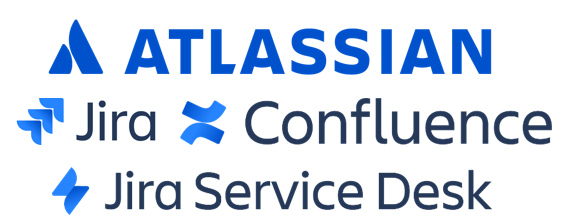
\includegraphics[width=.7\textwidth]{resources/atlassian_logo}\\
	\caption{The logos of \textit{Atlassian}, \textit{Jira}, \textit{Confluence} and \textit{Jira Service Desk}}
\end{figure}

%todo aggiungere issue tracking system a glossario
Jira is a proprietary Issue Tracking System was first released in 2002, the product name is a truncation of \textit{Gojira}, the Japanese word for Godzilla. This is a reference to another IST that was dominating the market, which is Bugzilla.
% https://www.workzone.com/blog/jira-alternatives/
Now the competitors of Jira are software like, for example, Redmine, VersionOne, PivotalTracker, Workzone or integrated ISTs in repositories like GitHub's or GitLab's issue trackers.
Athonet's choice has been Redmine because it's open source (this implies it's free of commision), it has a medium large community behind it and the plugins allow to integrate it with other internal tools used for issue tracking.

\begin{figure}[H]
	\centering
	
\includegraphics[width=.4\textwidth]{resources/redmine_logo}\\
	\caption{\textit{Redmine}'s logo}
\end{figure}

%todo aggiungere wiki a glossario
Confluence, on the other hand, is designed as a collaboration platform for sharing knowledge
%https://en.wikipedia.org/wiki/Confluence_(software)
Atlassian released Confluence 1.0 on March 25, 2004, saying its purpose was to build "an application that was built to the requirements of an enterprise knowledge management system, without losing the essential, powerful simplicity of the wiki in the process."

Like Jira, it's a proprietary tool the first version was released in 2004.

Both Jira and Confluence are written in Java

Othe than these tools Atlassian has acquired / developed other tools like Bamboo, Clover, Crowd, Crucible, and FishEye.

\section{Understanding what they can do}
These tools are made to be integrated with one another, not only because they are made by the same company but because they play well together.
Integrating an Issue Tracking with a platform able to share documents and thoughts
a cosa serve ciascuno (grafici o tabelle con funzionalità)\\
%http://www.akeles.com/what-are-the-differences-between-jira-software-jira-service-desk-and-jira-core/
si possono installare plugin
% licensing
	
	%https://www.atlassian.com/software/jira/guides/getting-started/overview#key-terms-to-know
	\subsection{Jira}
	
		At first it was just jira, then it specialized
	
		%todo aggiungere piccolo logo dei progetti vicino a ciascun titolo
		\subsubsection{Jira Core}
			Jira Core's main purpose is to handle business processes 
			
		\subsubsection{Jira Software}
			Jira Software's main purpose is to ho handle software projects
		
		\subsubsection{Jira Service desk}
			Jira Service desk's main purpose is to handle customer requests

		%https://marketplace.atlassian.com/apps/1212136/portfolio-for-jira/version-history
		\subsubsection{Jira Portfolio Plugin}
			Jira Portfolio was first designed as a plugin from ... then it was acquired by atlassian becaues
			It's main purpose is to visualize project roadmaps
		
	\subsection{Confluence}
		A

\section{How they can satisfy Athonet's needs}
come mai sono stati scelti proprio questi tool\\
descrivere cos'è la roadmap, perchè è così importante e perchè gli servono\\
cosa riescono a fare in più rispetto a quelli attuali\\
l'importanza di questi tool
		
	\subsection{Internal documentation}
		wiki

\section{How will Athonet use these tools}

	These tools are very complex, it is necessary to understand the scenario they can be used in and how the

	\subsection{Development} 
		Better tracking of inte
	
	\subsection{Management} 
		A
	
	\subsection{Client interaction} 
		A
		
	\subsection{Internal documentations}
		To be used as a wiki containing all the information for the employees
		
	\subsection{The difference between these and other internal tool}
		Sharepoint, otrs, office 365
		
		impossibile sostituire certi tool come word per la creazione di documenti per la condivizione con clienti / utenti ma sì per documentazione e wiki interna


riprendere necessità dell'azienda\\
fare un paio di uml con le varie figure aziendali e con cosa si andranno ad interfacciare

\section{The Atlassian Community}
	Choosing Jira and Confluence over other tools and implementing a brand new solution aka internally built software (reinventing the wheel) 
	because of the large community behind these tools.
	Atlassian offers a dedicated blog for Q\&A
	There are projects open in Jira online dedicated for Jira and Confluence, allowing users to open tickets and request for new features, report bugs etc.
	This allowed me to find information faster and 
